%Chapter 1 FTBS method

%\chapter{FTBS}

The first method to be explored is FTBS. Characteristics of the method can be found in \cite{mpebook}.
FTBS has been chosen as "naive" method to be compared to a more "sophisticathed" method and show the quantitative and qualitative differences.
The initial conditions used are the following:
\begin{equation}
\phi_0(t)=\left\{
\begin{array}{lr}
\frac{1}{2}(1-cos(4\pi x)) & 0\leq x<\frac{1}{2} \\
0 &  \frac{1}{2}\leq x\leq 1 \\
\end{array}
\right.
\label{eq:initcondcos}
\end{equation}

\begin{equation}
\phi_0(t)=\left\{
\begin{array}{lr}
1 & 0<x<\frac{1}{2} \\
0 &  elsewhere \\
\end{array}
\right.
\label{eq:initcondsquare}
\end{equation}
The function (\ref{eq:initcondcos}) can be used when smooth functions are needed, for example to test order of convergence. On the other hand, function with discontinuities, like the step function (\ref{eq:initcondsquare}) can be used to check monotonicity of the scheme.

\section{General characteristics}
We will explore the characteristics of the FTBS method. Unless otherwise stated, the results used in this chapter will be taken without proof from \cite{mpebook} and \cite{nmnotes}. 

\subsection{Conservation of mass} \label{conservationftbs}
With reference to equation (\ref{eq:linadvec_initcondition}), the mass of $\phi$ is conserved under the linear advection in the exact solution and also in the FTBS numerical implementation, whereas the variance of $\phi$ is conserved only in the exact solution but not in the FTBS implementation. The variance decreases in FTBS, and this is consistent with what we will find in the subsection \ref{stabilityftbs}, that the method is damping.

\subsection{Stability} \label{stabilityftbs}

\subsection{Accuracy}
The FTBS method is first order accurate. We can see in figure \ref{fig:ftbsvsexact} a qualitative comparison of the output of FTBS scheme vs the exact solution, for initial condition (\ref{eq:initcondcos}).
\begin{figure}[H]
	\begin{center}
		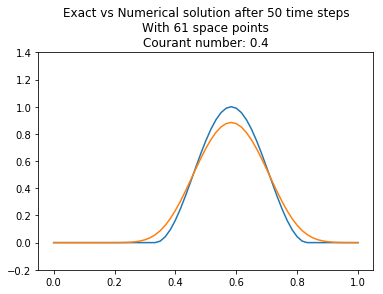
\includegraphics[width=4in]{graphics/FTBS_vs_exact.png}
	\end{center}%
	\caption[A comparison of FTBS vs exact solution.]{ \em A comparison of FTBS vs exact solution for initial condition (\ref{eq:initcondcos}). The blue line is the exact solution, the orange line is the output of the model}
	\label{fig:ftbsvsexact}
\end{figure}

\subsection{Monotonicity}
The FTBS is monotonic, it does not add new maxima, it can be seen qualitatively from figure \ref{fig:ftbsvsexact}.

\subsection{Dispersion errors}

\subsection{Diffusion errors}

\subsection{Computational modes}
What are these??? I read they refer to nothing specifically, but in general to modes that can be either physical or coming from numerical implementations. Not sure I understood how to compute these.

\subsection{Computational Cost}
Details of the code used for computing the FTBS scheme can be found in \ref{chap:pythonimplementation}.

\subsection{Variable resolution}
What does this mean specifically???
